%% Source: https://github.com/tias/constraint-solving-course
%% Licensed under CC BY-NC-SA 4.0: https://creativecommons.org/licenses/by-nc-sa/4.0/
%% You may share and adapt this for non-commercial use,
%% with attribution and under the same license.

\documentclass{cons-beamer}

\begin{document}


\begin{frame}{L07: Solving technologies and encodings}
  \begin{center}
    ~ \\
    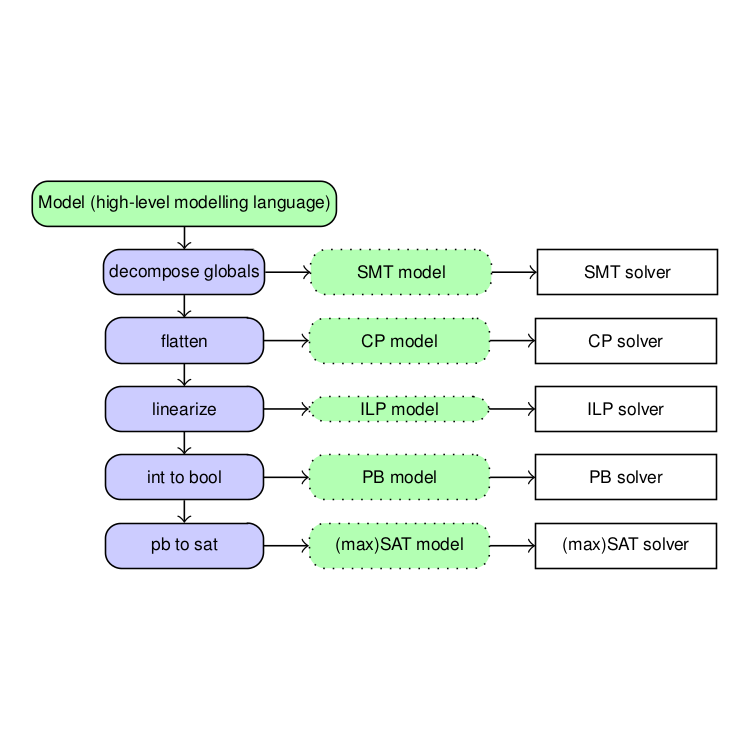
\includegraphics[height=42mm, trim=0 50pt 0 50pt, clip]{images/ch6-logo.png} \\
    Prof. Tias Guns and Dr. Dimos Tsouros \\[0.5em]
    
\includegraphics[width=2cm]{images/kuleuven_CMYK_logo.pdf}
  \end{center}
  
  {\footnotesize 
  Partly based on slides from Pierre Flener, Uppsala University.}
  % https://pierre-flener.github.io/courses/M4CO/lectures.html
\end{frame}

\begin{frame}{Solvers}
  You formulated a combinatorial problem in a high-level modeling language...
  \vfill 

  Now, \textit{which solver} should you use?
  \vfill

  %Solvers differ in:
  %\begin{itemize}
  %    \item The constraints they support (including global constraints/functions)
  %    \item The decision variables types they support (Boolean, integer, float, set, ...)
  %    \item How they perform search and propagation (CP vs MIP vs PB vs SAT)
  %    \item How they guide the search (heuristics, hyper-parameters)
  %\end{itemize}
\end{frame}

\begin{frame}
  \begin{examples}[Solving technologies]
    With general-purpose solvers, taking model and data as input:
    \begin{itemize}
      \item Boolean satisfiability (SAT)
      \item Pseudo-Boolean solving (PB)
      \item (Mixed) Integer Linear Programming (IP and MIP)
      \item SAT (resp.\ optimisation) Modulo Theories (SMT and OMT)
      \item Constraint programming (CP)
      \item \dots
    \end{itemize}
  \end{examples}
  \begin{examples}[Methodologies, \emph{usually without} modelling and solvers]
    \begin{itemize}
      \item Dynamic programming (DP)
      \item Greedy algorithms
      \item Local search (LS)
      \item Genetic algorithms (GA)
      \item \dots
    \end{itemize}
  \end{examples}
\end{frame}

\begin{frame}{How to Compare Solving Technologies?}
  \structured{Specification language:}
  \begin{itemize}
    \item What types of decision variables are available?  %  (Bool, int, float, string, ...)
    \item What types of constraints are available?  %  (clause, linear, alldifferent, ...)
    \item Can there be an objective function?
  \end{itemize}
  \vfill

  \structured{Guarantees:}
  \begin{itemize}
    \item Are its solvers \defined{exact}, given enough time: \\ will
      they prove unsatisfiability? prove optimality? find all solutions?
    \item If not, is there an \defined{approximation} ratio for the
      solution quality?
  \end{itemize}
  \vfill

  \structured{Features:}
  \begin{itemize}
    \item In which application areas has the technology been
      successfully used?
    \item Does the solving technology align well with this type of problem?
    \item Can the modeller influence the search process?  If yes, then how?
  \end{itemize}
\end{frame}

\begin{frame}{How Do Solvers Work? (Hooker, 2012)}
  \begin{definition}[Solving = Search + Inference + Relaxation]
    \begin{itemize}
      \item \search{Search}: Explore the space of candidate solutions.
      \item \inference{Inference}: Reduce the space of candidate solutions.
      \item \relaxation{Relaxation}: Exploit solutions to easier problems.
    \end{itemize}
  \end{definition}
  \vfill

  \begin{definition}[Systematic \search{Search}]
    Progressively build a solution, and backtrack if necessary. \\ Use
    \inference{inference} and \relaxation{relaxation} to reduce the
    search effort.
  \end{definition} \vfill
  Systematic search is used in most SMT, CP, ILP/MIP, PB and SAT solvers.
\end{frame}


\begin{frame}{How to model in a specific solvers' input language?}
  Every solver has their own input language.
  \vfill

  Different communities have different 'standard' input languages.
  \begin{itemize}
    \item SAT: DIMACS format
    \item Pseudo-Boolean: OPB format
    \item ILP/MIP: MPS format
    \item SMT: SMT-LIB format
  \end{itemize}
  \vspace{1em}

  The CP community does not really have a standard input language (due to the large variety of global constraints possible), BUT it has: \\
  \textbf{solver-independent modelling languages}
  \vfill

  How to go from a high-level modelling language to a specific solver input? Through transformations...
\end{frame}

\begin{frame}{From Model to Model to Solver: transformations}
\begin{tikzpicture}[scale=0.8, every node/.style={transform shape}, node distance=0.5cm]

% Model (green box)
\node[draw, fill=green!30, rounded corners, minimum width=2cm, minimum height=1cm] (model) {Model  (high-level modelling language)};

% Decompose-globals (blue box)
\node[draw, fill=blue!20, below=of model, rounded corners, minimum width=3.5cm, minimum height=1cm] (decompose) {decompose globals};
% Flatten (orange box)
\node[draw, fill=blue!20, below=of decompose, rounded corners, minimum width=3.5cm, minimum height=1cm] (flatten) {flatten};
% Linearize (purple box)
\node[draw, fill=blue!20, below=of flatten, rounded corners, minimum width=3.5cm, minimum height=1cm] (linearize) {linearize};
% int2bool (cyan box)
\node[draw, fill=blue!20, below=of linearize, rounded corners, minimum width=3.5cm, minimum height=1cm] (int2bool) {int to bool};
% pb2sat (pink box)
\node[draw, fill=blue!20, below=of int2bool, rounded corners, minimum width=3.5cm, minimum height=1cm] (pb2sat) {pb to sat};

% Low-level mdoels (no fill)
\node[draw, fill=green!30, rounded corners, dotted, minimum height=1cm, minimum width=4cm, right=1cm of decompose, align=left] (smt) {SMT model};
\node[draw, fill=green!30, rounded corners, dotted, minimum height=1cm, minimum width=4cm, right=1cm of flatten, align=left] (cp) {CP model};
\node[draw, fill=green!30, rounded corners, dotted, minimum width=4cm, right=1cm of linearize, fill=green!30, rounded corners, align=left] (ilp) {ILP model};
\node[draw, fill=green!30, rounded corners, dotted, minimum height=1cm, minimum width=4cm, right=1cm of int2bool, align=left] (pb) {PB model};
\node[draw, fill=green!30, rounded corners, dotted, minimum height=1cm, minimum width=4cm, right=1cm of pb2sat, align=left] (sat) {(max)SAT model};

% Solvers (no fill)
\node[draw, minimum height=1cm, minimum width=4cm, right=1cm of smt, align=left] (smt2) {SMT solver};
\node[draw, minimum height=1cm, minimum width=4cm, right=1cm of cp, align=left] (cp2) {CP solver};
\node[draw, minimum height=1cm, minimum width=4cm, right=1cm of ilp, align=left] (ilp2) {ILP solver};
\node[draw, minimum height=1cm, minimum width=4cm, right=1cm of pb, align=left] (pb2) {PB solver};
\node[draw, minimum height=1cm, minimum width=4cm, right=1cm of sat, align=left] (sat2) {(max)SAT solver};

% Arrows
\draw[->] (model) -- (decompose); 
\draw[->] (decompose) -- (flatten);
\draw[->] (flatten) -- (linearize);
\draw[->] (linearize) -- (int2bool);
\draw[->] (int2bool) -- (pb2sat);

% Connections to low-level
\draw[->] (decompose.east) -- ++(0.5,0) |- (smt.west);
\draw[->] (flatten.east) -- ++(0.5,0) |- (cp.west);
\draw[->] (linearize.east) -- ++(0.5,0) |- (ilp.west);
\draw[->] (int2bool.east) -- ++(0.5,0) |- (pb.west);
\draw[->] (pb2sat.east) -- ++(0.5,0) |- (sat.west);

% Connections to solvers
\draw[->] (smt.east) -- ++(0.5,0) |- (smt2.west);
\draw[->] (cp.east) -- ++(0.5,0) |- (cp2.west);
\draw[->] (ilp.east) -- ++(0.5,0) |- (ilp2.west);
\draw[->] (pb.east) -- ++(0.5,0) |- (pb2.west);
\draw[->] (sat.east) -- ++(0.5,0) |- (sat2.west);

\end{tikzpicture}
\end{frame}


\begin{frame}{Objectives}
  An overview of some solving technologies: \vfill
  \begin{itemize}
    \item to understand their advantages and limitations; \vfill
    \item to help you choose a technology for a particular model; \vfill
    \item to help you encode and adapt a model to a particular technology.
  \end{itemize}
\end{frame}


\section*{Solvers}

\subsection*{SAT Modulo Theories (SMT)}


% OVERVIEW: SMT solver highlight
\begin{frame}{Overview}
\begin{tikzpicture}[scale=0.7, every node/.style={transform shape}, node distance=0.5cm]

% Model (green box)
\node[draw, fill=green!30, rounded corners, minimum width=2cm, minimum height=1cm] (model) {Model  (high-level modelling language)};

% Decompose-globals (blue box)
\node[draw, fill=blue!20, below=of model, rounded corners, minimum width=3.5cm, minimum height=1cm] (decompose) {decompose globals};
% Flatten (orange box)
\node[draw, fill=blue!20, below=of decompose, rounded corners, minimum width=3.5cm, minimum height=1cm] (flatten) {flatten};
% Linearize (purple box)
\node[draw, fill=blue!20, below=of flatten, rounded corners, minimum width=3.5cm, minimum height=1cm] (linearize) {linearize};
% int2bool (cyan box)
\node[draw, fill=blue!20, below=of linearize, rounded corners, minimum width=3.5cm, minimum height=1cm] (int2bool) {int to bool};
% pb2sat (pink box)
\node[draw, fill=blue!20, below=of int2bool, rounded corners, minimum width=3.5cm, minimum height=1cm] (pb2sat) {pb to sat};

% Low-level mdoels (no fill)
\node[draw, fill=green!30, rounded corners, dotted, minimum height=1cm, minimum width=4cm, right=1cm of decompose, align=left] (smt) {SMT model};
\node[draw, fill=green!30, rounded corners, dotted, minimum height=1cm, minimum width=4cm, right=1cm of flatten, align=left] (cp) {CP model};
\node[draw, fill=green!30, rounded corners, dotted, minimum width=4cm, right=1cm of linearize, fill=green!30, rounded corners, align=left] (ilp) {ILP model};
\node[draw, fill=green!30, rounded corners, dotted, minimum height=1cm, minimum width=4cm, right=1cm of int2bool, align=left] (pb) {PB model};
\node[draw, fill=green!30, rounded corners, dotted, minimum height=1cm, minimum width=4cm, right=1cm of pb2sat, align=left] (sat) {(max)SAT model};

% Solvers (no fill)
\node[draw, fill=red!30, minimum height=1cm, minimum width=4cm, right=1cm of smt, align=left] (smt2) {SMT solver};
\node[draw, minimum height=1cm, minimum width=4cm, right=1cm of cp, align=left] (cp2) {CP solver};
\node[draw, minimum height=1cm, minimum width=4cm, right=1cm of ilp, align=left] (ilp2) {ILP solver};
\node[draw, minimum height=1cm, minimum width=4cm, right=1cm of pb, align=left] (pb2) {PB solver};
\node[draw, minimum height=1cm, minimum width=4cm, right=1cm of sat, align=left] (sat2) {(max)SAT solver};

% Arrows
\draw[->] (model) -- (decompose); 
\draw[->] (decompose) -- (flatten);
\draw[->] (flatten) -- (linearize);
\draw[->] (linearize) -- (int2bool);
\draw[->] (int2bool) -- (pb2sat);

% Connections to low-level
\draw[->] (decompose.east) -- ++(0.5,0) |- (smt.west);
\draw[->] (flatten.east) -- ++(0.5,0) |- (cp.west);
\draw[->] (linearize.east) -- ++(0.5,0) |- (ilp.west);
\draw[->] (int2bool.east) -- ++(0.5,0) |- (pb.west);
\draw[->] (pb2sat.east) -- ++(0.5,0) |- (sat.west);

% Connections to solvers
\draw[->] (smt.east) -- ++(0.5,0) |- (smt2.west);
\draw[->] (cp.east) -- ++(0.5,0) |- (cp2.west);
\draw[->] (ilp.east) -- ++(0.5,0) |- (ilp2.west);
\draw[->] (pb.east) -- ++(0.5,0) |- (pb2.west);
\draw[->] (sat.east) -- ++(0.5,0) |- (sat2.west);

\end{tikzpicture}
\end{frame}


\begin{frame}[fragile]{SAT Modulo Theories (SMT) and OMT}
  \structured{Modelling Language:}
  \begin{itemize}
    \item Language of SAT: Boolean decision variables and clauses.
    \item Several \defined{theories} extend the language, such as \\ bit vectors,
      uninterpreted functions, or linear integer arithmetic.
    \item SMT is only for satisfaction problems.
    \item OMT (optimisation modulo theories) extends SMT.
  \end{itemize}
  \begin{definition}
    A \defined{theory}
    \begin{itemize}
      \item defines types for decision variables and defines constraint
        predicates;
      \item is associated with a sub-solver for any conjunction of its
        predicates.
    \end{itemize}
  \end{definition}
  Different SMT or OMT solvers may have different theories.
\end{frame}

\begin{frame}{LIA}
  Example: \defined{theory} of Linear Integer Arithmetic (LIA)
  (variables can be unbounded for SMT solvers!)
  \vfill

  \begin{columns}
    \begin{column}{0.45\textwidth}
      \textbf{Mathematical Formulation}
      \begin{align*}
        & (x \geq 0)\\
        & (y \leq 0) \\
        & (x = y + 1) \lor (x = 2 \cdot y) \\
        & (x = 2) \lor (y = -2) \lor (x = y)
      \end{align*}
    \end{column}
    \begin{column}{0.45\textwidth}
      \textbf{SMT-LIB format}
      \begin{align*}
        &\texttt{(>= x 0)}\\
        &\texttt{(<= y 0)}\\
        &\texttt{(or (= x (+ y 1)) (= x (* 2 y)))}\\
        &\texttt{(or (= x 2) (= y -2) (= x y))}
      \end{align*}
    \end{column}
  \end{columns}
\end{frame}

\begin{frame}{Satisfiability Modulo Theories (SMT)}
  \begin{itemize}
    %\item Extends \textbf{SAT} (Boolean Satisfiability) by adding rich background \textbf{theories} \\(e.g., arithmetic, arrays, bit-vectors, strings, uninterpreted functions).
    \item Determines the satisfiability of a first-order logical formulas over (one or more) background theories
    \item if SAT: return SAT + a solution to the \emph{theory} problem\\
          if UNSAT: return UNSAT
    \item there is a standardized language for many different theories, that all SMT solvers accept: the SMT-LIB language
  \end{itemize}
  \vfill

  \textbf{Typical application areas}
  \begin{itemize}
    \item {Formal Verification} of hardware and software
    \item {Model Checking}, and {Program Analysis}
    \item {Automated Reasoning}, {Theorem Proving}
  \end{itemize}
\end{frame}

\begin{frame}{Boolean abstraction}
  Separate the theory constraints and create the Boolean skeleton
  \vfill

  Example:
  \begin{align*}
    & (x \geq 0) \land (y \leq 0) \\
    & (x = y + 1) \lor (x = 2 \cdot y) \\
    & (x = 2) \lor (y = -2) \lor (x = y)
  \end{align*}

  Boolean skeleton:
  $a \land b \land (c \lor d) \land (e \lor f \lor g)$

  Theory constraints (each Boolean indicates whether a constraint holds or not):
  \begin{align*}
    &a \leftrightarrow (x \geq 0) \land b \leftrightarrow y \leq 0) \land \\
    &c \leftrightarrow (x = y + 1) \land d \leftrightarrow (x = 2 * y) \land \\
    &e \leftrightarrow (x = 2) \land f \leftrightarrow (y = -2) \land g \leftrightarrow (x = y)
  \end{align*}
\end{frame}

\begin{frame}{SMT Solving: DPLL($T$\,)}
  \textbf{How it Works (High-Level Overview)} $ $\\
  Combines a SAT solver with a theory solver.
  \begin{itemize}
    \item \textbf{SAT solver} generates Boolean assignment over the Boolean skeleton;
    \item \textbf{Theory solver} checks consistency of activated theory constraints; \\
    \begin{itemize}
      \item if SAT: generate theory-level assignment, return
      \item if UNSAT: generate Boolean-level \textit{conflict} between theory constraints, add it to the SAT solver
    \end{itemize}
    \item repeat.
  \end{itemize}
  \vfill

  Theory solvers operate over all (activated) constraints in the theory at once. 
  Efficient theory solvers are incremental: reuse information from previous checks.
  \vfill

  Example SMT solvers: 
    \href{https://cvc4.github.io}{CVC4},
    \href{https://yices.csl.sri.com}{Yices 2},
    \href{https://github.com/Z3Prover/z3}{Z3}, \dots

  Example OMT solvers:
    \href{https://optimathsat.disi.unitn.it}{OptiMathSAT},
    \href{https://github.com/Z3Prover/z3}{Z3}
\end{frame}

\begin{frame}{SMT/OMT for CP solving}
  Theory: QF\_LIA = "Quantifier Free, Linear Integer Arithmetic"
  (and QF\_NIA in case of non-linearities)
  \vfill

  Supports Bool and Int, as well as logical and arithmetic operators; including nested expressions thereof.
  \vfill

  But no global constraints / global functions:
  \begin{itemize}
    \item requires to \defined{decompose} global constraints
  \end{itemize}
\end{frame}


\subsection*{Transformation: decompose}
\begin{frame}{Overview}
\begin{tikzpicture}[scale=0.7, every node/.style={transform shape}, node distance=0.5cm]

% Model (green box)
\node[draw, fill=green!30, rounded corners, minimum width=2cm, minimum height=1cm] (model) {Model  (high-level modelling language)};

% Decompose-globals (blue box)
\node[draw, fill=red!30, below=of model, rounded corners, minimum width=3.5cm, minimum height=1cm] (decompose) {decompose globals};
% Flatten (orange box)
\node[draw, fill=blue!20, below=of decompose, rounded corners, minimum width=3.5cm, minimum height=1cm] (flatten) {flatten};
% Linearize (purple box)
\node[draw, fill=blue!20, below=of flatten, rounded corners, minimum width=3.5cm, minimum height=1cm] (linearize) {linearize};
% int2bool (cyan box)
\node[draw, fill=blue!20, below=of linearize, rounded corners, minimum width=3.5cm, minimum height=1cm] (int2bool) {int to bool};
% pb2sat (pink box)
\node[draw, fill=blue!20, below=of int2bool, rounded corners, minimum width=3.5cm, minimum height=1cm] (pb2sat) {pb to sat};

% Low-level mdoels (no fill)
\node[draw, fill=green!30, rounded corners, dotted, minimum height=1cm, minimum width=4cm, right=1cm of decompose, align=left] (smt) {SMT model};
\node[draw, fill=green!30, rounded corners, dotted, minimum height=1cm, minimum width=4cm, right=1cm of flatten, align=left] (cp) {CP model};
\node[draw, fill=green!30, rounded corners, dotted, minimum width=4cm, right=1cm of linearize, fill=green!30, rounded corners, align=left] (ilp) {ILP model};
\node[draw, fill=green!30, rounded corners, dotted, minimum height=1cm, minimum width=4cm, right=1cm of int2bool, align=left] (pb) {PB model};
\node[draw, fill=green!30, rounded corners, dotted, minimum height=1cm, minimum width=4cm, right=1cm of pb2sat, align=left] (sat) {(max)SAT model};

% Solvers (no fill)
\node[draw, minimum height=1cm, minimum width=4cm, right=1cm of smt, align=left] (smt2) {SMT solver};
\node[draw, minimum height=1cm, minimum width=4cm, right=1cm of cp, align=left] (cp2) {CP solver};
\node[draw, minimum height=1cm, minimum width=4cm, right=1cm of ilp, align=left] (ilp2) {ILP solver};
\node[draw, minimum height=1cm, minimum width=4cm, right=1cm of pb, align=left] (pb2) {PB solver};
\node[draw, minimum height=1cm, minimum width=4cm, right=1cm of sat, align=left] (sat2) {(max)SAT solver};

% Arrows
\draw[->] (model) -- (decompose); 
\draw[->] (decompose) -- (flatten);
\draw[->] (flatten) -- (linearize);
\draw[->] (linearize) -- (int2bool);
\draw[->] (int2bool) -- (pb2sat);

% Connections to low-level
\draw[->] (decompose.east) -- ++(0.5,0) |- (smt.west);
\draw[->] (flatten.east) -- ++(0.5,0) |- (cp.west);
\draw[->] (linearize.east) -- ++(0.5,0) |- (ilp.west);
\draw[->] (int2bool.east) -- ++(0.5,0) |- (pb.west);
\draw[->] (pb2sat.east) -- ++(0.5,0) |- (sat.west);

% Connections to solvers
\draw[->] (smt.east) -- ++(0.5,0) |- (smt2.west);
\draw[->] (cp.east) -- ++(0.5,0) |- (cp2.west);
\draw[->] (ilp.east) -- ++(0.5,0) |- (ilp2.west);
\draw[->] (pb.east) -- ++(0.5,0) |- (pb2.west);
\draw[->] (sat.east) -- ++(0.5,0) |- (sat2.west);

\end{tikzpicture}
\end{frame}


\begin{frame}{Decomposing global constraints}
  \small
  Rewrite global constraints using (more) primitive constraints.

  \begin{example}
    \small
    $\cons{AllDifferent}{x_1, \dots, x_n}$:
    Its decomposition is a conjunction of
    $\frac{n\cdot(n-1)}{2}$ disequality
    constraints:
    \vspace{-3mm}
    \[
    \bigwedge_{i, j \in \{1..n\}, i < j} x_i \neq x_j
    \]
  \end{example}

  \begin{example}
    \small
    \cons{Cumulative}{s,d,r,c}:
    Its time-resource decomposition introduces new Booleans \( B_{it} \), representing if task \( i \) (with start time $s_i$, and duration $d_i$) is active at time \( t \):
    \vspace{-3mm}
    \[
    \forall t \in \{0..t_{\text{max}} - 1\}, \forall i \in \{1..n\} : \quad B_{it} \leftrightarrow (s_i \leq t) \land \neg(s_i \leq t - d_i)
    \]

    The resource constraint at each time \( t \), for $n$ tasks, with $r_i$ being the resource consumption of task $i$, is expressed as:
    \vspace{-3mm}
    \[
    \forall t \in \{0..t_{\text{max}} - 1\} : \quad \sum_{i \in [1..n]} r_i \cdot B_{it} \leq c
    \]
    \vspace{-3mm}
  \end{example}
\end{frame}

\begin{frame}{Decomposing global functions}
  \small
  The function itself is an integer-valued function. Need to decompose wrt a specific comparison.

  \begin{example}
    $\cons{Count}{A, v} == res$ (or $\cons{CountEq}{A,v,res}$): Its decomposition is a sum constraint over all variables:
      \[
      \sum_{i}  [ A_i = v ]  = res
      \]
  \end{example}

  \begin{example}
    $\cons{Element}{Arr, idx} == res$ (or $\cons{ElementEq}{Arr, idx, res}$, or $Arr[idx] == res$): Its decomposition is a list of implications, specifying that if the index has a given value, then the respective value from the array must be equal to the resulting variable $res$:
      \[
      \forall i \in \{0..n - 1\}, \quad (\text{idx} = i) \rightarrow (\text{Arr}_i \ = \ \text{res})
      \]
  \end{example}

\end{frame}

\subsection*{Constraint Programming (CP)}
% OVERVIEW: CP solver highlight
\begin{frame}{Overview}
\begin{tikzpicture}[scale=0.7, every node/.style={transform shape}, node distance=0.5cm]

% Model (green box)
\node[draw, fill=green!30, rounded corners, minimum width=2cm, minimum height=1cm] (model) {Model  (high-level modelling language)};

% Decompose-globals (blue box)
\node[draw, fill=blue!20, below=of model, rounded corners, minimum width=3.5cm, minimum height=1cm] (decompose) {decompose globals};
% Flatten (orange box)
\node[draw, fill=blue!20, below=of decompose, rounded corners, minimum width=3.5cm, minimum height=1cm] (flatten) {flatten};
% Linearize (purple box)
\node[draw, fill=blue!20, below=of flatten, rounded corners, minimum width=3.5cm, minimum height=1cm] (linearize) {linearize};
% int2bool (cyan box)
\node[draw, fill=blue!20, below=of linearize, rounded corners, minimum width=3.5cm, minimum height=1cm] (int2bool) {int to bool};
% pb2sat (pink box)
\node[draw, fill=blue!20, below=of int2bool, rounded corners, minimum width=3.5cm, minimum height=1cm] (pb2sat) {pb to sat};

% Low-level mdoels (no fill)
\node[draw, fill=green!30, rounded corners, dotted, minimum height=1cm, minimum width=4cm, right=1cm of decompose, align=left] (smt) {SMT model};
\node[draw, fill=green!30, rounded corners, dotted, minimum height=1cm, minimum width=4cm, right=1cm of flatten, align=left] (cp) {CP model};
\node[draw, fill=green!30, rounded corners, dotted, minimum width=4cm, right=1cm of linearize, fill=green!30, rounded corners, align=left] (ilp) {ILP model};
\node[draw, fill=green!30, rounded corners, dotted, minimum height=1cm, minimum width=4cm, right=1cm of int2bool, align=left] (pb) {PB model};
\node[draw, fill=green!30, rounded corners, dotted, minimum height=1cm, minimum width=4cm, right=1cm of pb2sat, align=left] (sat) {(max)SAT model};

% Solvers (no fill)
\node[draw, minimum height=1cm, minimum width=4cm, right=1cm of smt, align=left] (smt2) {SMT solver};
\node[draw, fill=red!30, minimum height=1cm, minimum width=4cm, right=1cm of cp, align=left] (cp2) {CP solver};
\node[draw, minimum height=1cm, minimum width=4cm, right=1cm of ilp, align=left] (ilp2) {ILP solver};
\node[draw, minimum height=1cm, minimum width=4cm, right=1cm of pb, align=left] (pb2) {PB solver};
\node[draw, minimum height=1cm, minimum width=4cm, right=1cm of sat, align=left] (sat2) {(max)SAT solver};

% Arrows
\draw[->] (model) -- (decompose); 
\draw[->] (decompose) -- (flatten);
\draw[->] (flatten) -- (linearize);
\draw[->] (linearize) -- (int2bool);
\draw[->] (int2bool) -- (pb2sat);

% Connections to low-level
\draw[->] (decompose.east) -- ++(0.5,0) |- (smt.west);
\draw[->] (flatten.east) -- ++(0.5,0) |- (cp.west);
\draw[->] (linearize.east) -- ++(0.5,0) |- (ilp.west);
\draw[->] (int2bool.east) -- ++(0.5,0) |- (pb.west);
\draw[->] (pb2sat.east) -- ++(0.5,0) |- (sat.west);

% Connections to solvers
\draw[->] (smt.east) -- ++(0.5,0) |- (smt2.west);
\draw[->] (cp.east) -- ++(0.5,0) |- (cp2.west);
\draw[->] (ilp.east) -- ++(0.5,0) |- (ilp2.west);
\draw[->] (pb.east) -- ++(0.5,0) |- (pb2.west);
\draw[->] (sat.east) -- ++(0.5,0) |- (sat2.west);

\end{tikzpicture}
\end{frame}


\begin{frame}{Constraint Programming (CP)}
  \begin{itemize}
    \item Solves combinatorial optimisation problems with finite-domain variables
    \item Includes logical, arithmetic and specialised \textit{global constraints}
    \item Solves both satisfaction and optimisation problems
  \end{itemize}
  \vfill

  \textbf{How it Works (High-Level Overview)}  $ $\\
  \begin{itemize}
    \item \textbf{Propagation} each constraint reduces the domains of the variables involved as much as possible until no domain can be further reduced;
    \item \textbf{Systematic search} the solver chooses a variable and branches over each of its remaining values
  \end{itemize}
  \vfill

  \textbf{Typical Applications}
  \begin{itemize}
    \item Scheduling, Timetabling, Assignment problems
    \item Routing Problems, Packing problems, esp. with side-constraints
    \item Puzzles and Games, Configuration Problems
  \end{itemize}
\end{frame}

\begin{frame}{Constraint Programming (CP)}
  \structured{Modelling Language = flat list of (supported) constraints}
  \begin{itemize}
    \item Variables: Boolean, integer (finite-domain); a few solvers support sets, floats even graphs
    \item Logic, arithmetic and \textbf{global} constraints
    \item For satisfaction problems and optimisation problems.
  \end{itemize}
  \vfill

  \structured{Many solvers}
  There is no standard input format for CP solvers... two things come close:
  \begin{itemize}
    \item XCSP3: an XML format, contrary to most solvers it allows for some form of nesting and many global constraints
    \item FlatZinc: an intermediary 'flat' predicate list produced by MiniZinc, but creates multiple auxiliary variables and no standard constraint naming (can differ for different solvers) 
  \end{itemize}
\end{frame}

\begin{frame}{Domains}
  \begin{definition}
    The \defined{domain} of a decision variable $v$, denoted here by
    $\Domain{v}$, is the set of values that $v$ can still take during
    \search{search}:
    \begin{itemize}
      \item The domains of the decision variables are reduced by
        \search{search} \\ and by \inference{inference} (see the next two
        slides).
      \item A decision variable is said to be \defined{fixed} if its
        domain is a singleton.
      \item \defined{Unsatisfiability} occurs if the domain of a
        decision variable goes empty.
    \end{itemize}
  \end{definition}
  \vfill

  Note the difference between:
  \begin{itemize}
    \item a domain as a technology-independent declarative entity when
      modelling;
    \item a domain as a CP-technology procedural data structure when
      solving.
  \end{itemize}
\end{frame}

\begin{frame}{CP solver structure}
  \centering
  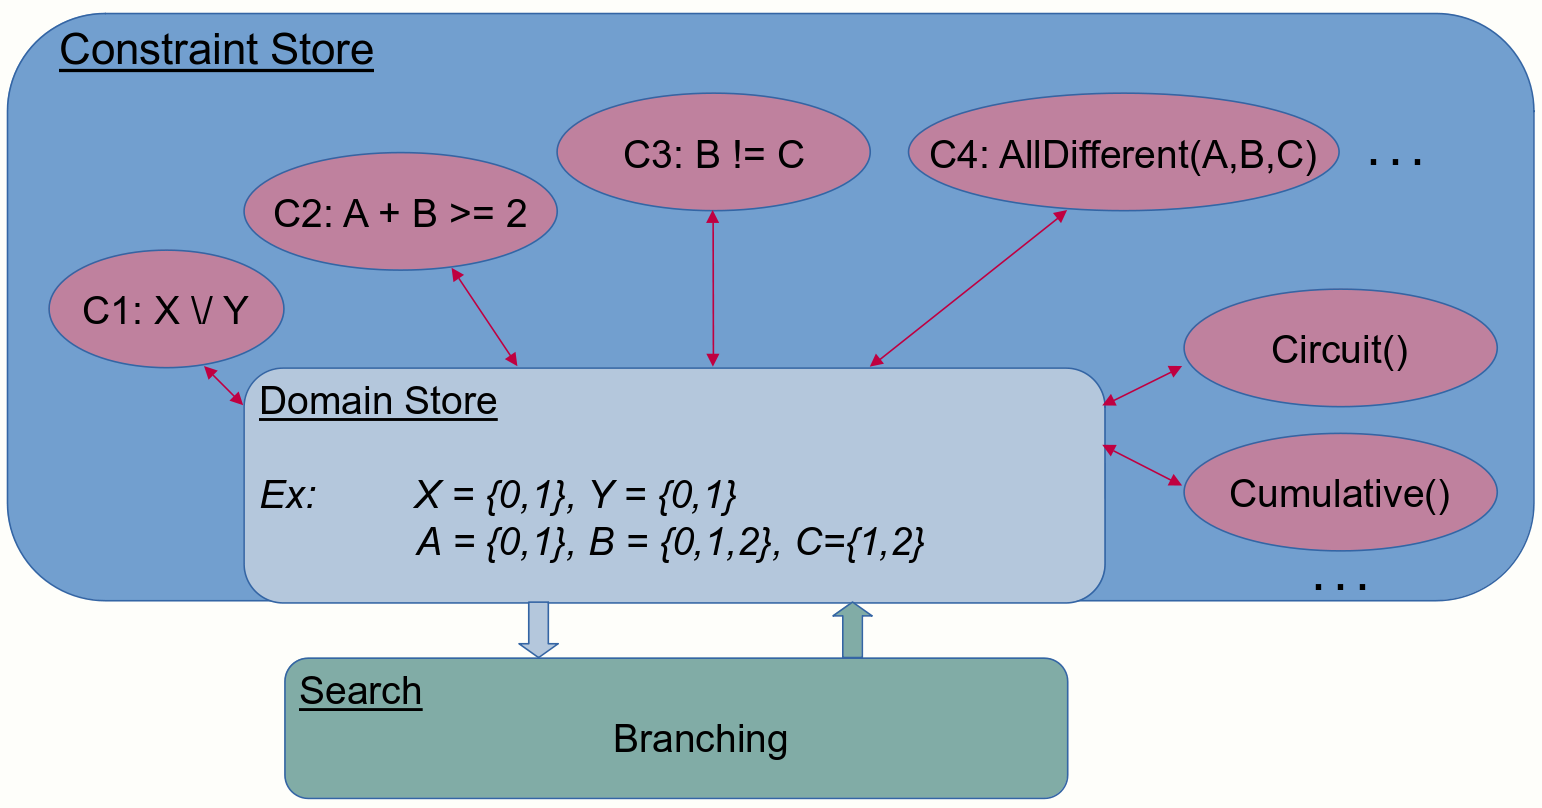
\includegraphics[height=70mm]{images/cp_domain_store.png}
\end{frame}

\begin{frame}{CP Solving}
  \search{Tree Search}, upon initialising each domain as in the model: \vfill

  \structured{Satisfaction problem}:
  \begin{enumerate}
    \item Perform propagation \inference{inference}.
    \item If the domain of some decision variable is empty, then
      backtrack.
    \item If all decision variables are fixed, then we have a solution.
    \item Select a non-fixed decision variable $v$, \\ partition its
      domain into two parts $\pi_1$ and $\pi_2$, and make two branches: \\
      one with $v \in \pi_1$, and the other one with $v \in \pi_2$.
    \item Recursively explore each of the two branches.
  \end{enumerate}
  \vfill

  \structured{Optimisation problem}: when a feasible solution is found
  at step~3, first add the constraint that the next solution must
  be better and then backtrack.
\end{frame}

\begin{frame}{CP Inference}
  \begin{definition}
    A \inference{propagator} for a constraint $\gamma$ deletes from the
    domains of the
    % decision
    variables of a~$\gamma$-constraint
    the values that cannot
    be in a solution to that constraint. \\
  \end{definition}
  \begin{examples}
    \begin{itemize}
      \item For $x < y$: when $\Domain{x} = \{1..4\}$ and $\Domain{y} = \{-1..3\}$,
        delete $\{3, 4\}$ from $\Domain{x}$ and
        $\{-1..1\}$ from $\Domain{y}$.
      \item For $\cons{AllDifferent}{x,y,z}$: when
        $\Domain{x} = \{1..3\}$ =
        $\Domain{y}$ and $\Domain{z} = \{1..4\}$, delete $1$ and $3$ from
        $\Domain{z}$ so that it becomes the non-range
        $\{2,4\}$.
    \end{itemize}
  \end{examples}

  Propagation of constraints is executed until \textbf{fixed-point}: no constraint can reduce the current domains further.
\end{frame}

\begin{frame}{Strategies and Improvements}
  \search{Search Strategies:}
  \begin{itemize}
    \item On which decision variable to branch next?
    \item How to partition the domain of the chosen decision variable?
    \item Which search (depth-first, breadth-first, \dots) to use?
  \end{itemize}
  \vfill

  \structured{Improvements:}
  \begin{itemize}
    \item \inference{Propagators}, including for global constraints and global functions. \\ Not all impossible domain values need to
      be deleted: there is a compromise between algorithm complexity and
      achieved \inference{inference}.
    \item \search{Partition} the chosen domain into at least two parts.
    \item Domain representations.
    \item \search{Order} in which propagators are executed (and re-actived when a variable changes)
    \item \dots
  \end{itemize}
\end{frame}

\begin{frame}{CP Solving}
  \begin{itemize}
    \item Guarantee: exact, given enough time. \vfill
    \item White-box: within a solver one can design one's own \inference{propagators}
      and \search{search strategies}, or choose among predefined ones.
      \vfill
    \item Successful application areas:
      \begin{itemize}
        \item Configuration
        \item Scheduling
        \item Personnel rostering and timetabling
        \item rich vehicle routing
        \item \dots
      \end{itemize}
  \end{itemize}
\end{frame}


\subsection*{Transformation: flatten}
\begin{frame}{Overview}
\begin{tikzpicture}[scale=0.7, every node/.style={transform shape}, node distance=0.5cm]

% Model (green box)
\node[draw, fill=green!30, rounded corners, minimum width=2cm, minimum height=1cm] (model) {Model  (high-level modelling language)};

% Decompose-globals (blue box)
\node[draw, fill=blue!20, below=of model, rounded corners, minimum width=3.5cm, minimum height=1cm] (decompose) {decompose globals};
% Flatten (orange box)
\node[draw, fill=red!30, below=of decompose, rounded corners, minimum width=3.5cm, minimum height=1cm] (flatten) {flatten};
% Linearize (purple box)
\node[draw, fill=blue!20, below=of flatten, rounded corners, minimum width=3.5cm, minimum height=1cm] (linearize) {linearize};
% int2bool (cyan box)
\node[draw, fill=blue!20, below=of linearize, rounded corners, minimum width=3.5cm, minimum height=1cm] (int2bool) {int to bool};
% pb2sat (pink box)
\node[draw, fill=blue!20, below=of int2bool, rounded corners, minimum width=3.5cm, minimum height=1cm] (pb2sat) {pb to sat};

% Low-level mdoels (no fill)
\node[draw, fill=green!30, rounded corners, dotted, minimum height=1cm, minimum width=4cm, right=1cm of decompose, align=left] (smt) {SMT model};
\node[draw, fill=green!30, rounded corners, dotted, minimum height=1cm, minimum width=4cm, right=1cm of flatten, align=left] (cp) {CP model};
\node[draw, fill=green!30, rounded corners, dotted, minimum width=4cm, right=1cm of linearize, fill=green!30, rounded corners, align=left] (ilp) {ILP model};
\node[draw, fill=green!30, rounded corners, dotted, minimum height=1cm, minimum width=4cm, right=1cm of int2bool, align=left] (pb) {PB model};
\node[draw, fill=green!30, rounded corners, dotted, minimum height=1cm, minimum width=4cm, right=1cm of pb2sat, align=left] (sat) {(max)SAT model};

% Solvers (no fill)
\node[draw, minimum height=1cm, minimum width=4cm, right=1cm of smt, align=left] (smt2) {SMT solver};
\node[draw, minimum height=1cm, minimum width=4cm, right=1cm of cp, align=left] (cp2) {CP solver};
\node[draw, minimum height=1cm, minimum width=4cm, right=1cm of ilp, align=left] (ilp2) {ILP solver};
\node[draw, minimum height=1cm, minimum width=4cm, right=1cm of pb, align=left] (pb2) {PB solver};
\node[draw, minimum height=1cm, minimum width=4cm, right=1cm of sat, align=left] (sat2) {(max)SAT solver};

% Arrows
\draw[->] (model) -- (decompose); 
\draw[->] (decompose) -- (flatten);
\draw[->] (flatten) -- (linearize);
\draw[->] (linearize) -- (int2bool);
\draw[->] (int2bool) -- (pb2sat);

% Connections to low-level
\draw[->] (decompose.east) -- ++(0.5,0) |- (smt.west);
\draw[->] (flatten.east) -- ++(0.5,0) |- (cp.west);
\draw[->] (linearize.east) -- ++(0.5,0) |- (ilp.west);
\draw[->] (int2bool.east) -- ++(0.5,0) |- (pb.west);
\draw[->] (pb2sat.east) -- ++(0.5,0) |- (sat.west);

% Connections to solvers
\draw[->] (smt.east) -- ++(0.5,0) |- (smt2.west);
\draw[->] (cp.east) -- ++(0.5,0) |- (cp2.west);
\draw[->] (ilp.east) -- ++(0.5,0) |- (ilp2.west);
\draw[->] (pb.east) -- ++(0.5,0) |- (pb2.west);
\draw[->] (sat.east) -- ++(0.5,0) |- (sat2.west);

\end{tikzpicture}
\end{frame}


\begin{frame}{From CP Language to CP Solver: flattening steps}
  \begin{enumerate}
    \item[0.] Decompose Unsupported Globals (see previous part)

    \item \textbf{Push down negation}
      \begin{itemize}
        \item Simplifies later code by eliminating 'negation' operator, \\afterwards only in front of Boolean variable
        \item Example: $\neg(x \land y)$ becomes $(\neg x \lor \neg y)$ and $\neg (a > b)$ becomes $(a \leq b)$
      \end{itemize}

    \item \textbf{Normalize and simplify expressions}
      \begin{itemize}
        \item Eliminates unnecessary 'nested' expressions, avoids auxiliary variables later
        \item Example: $(x \rightarrow (y \lor z))$ becomes $(\neg x \lor y \lor z)$ and $(a - (b + 2c))$ becomes $(a -b -2c)$
      \end{itemize}

    \item \textbf{Unnest arguments using auxiliary variables}
      \begin{itemize}
        \item Because CP solvers only accept a list of constraints over variables
        \item Example: Rewrite $x \lor (a + b \geq 2)$ by:
          \begin{itemize}
            \item Introduce auxiliary variable $w$ (here: Boolean)
            \item Add new constraint to solver: \( w = (a + b \geq 2) \)
            \item Rewrite $(x \lor (a + b \geq 2))$ to $(x \lor w)$
          \end{itemize}
        \item Similarly for $(a + (b*c) \geq 0)$: $(w = b*c) \land (a + w \geq 0)$
      \end{itemize}
  \end{enumerate}
\end{frame}


\subsection*{Integer Linear Programming (ILP)}
% OVERVIEW: ILP solver highlight
\begin{frame}{Overview}
\begin{tikzpicture}[scale=0.7, every node/.style={transform shape}, node distance=0.5cm]

% Model (green box)
\node[draw, fill=green!30, rounded corners, minimum width=2cm, minimum height=1cm] (model) {Model  (high-level modelling language)};

% Decompose-globals (blue box)
\node[draw, fill=blue!20, below=of model, rounded corners, minimum width=3.5cm, minimum height=1cm] (decompose) {decompose globals};
% Flatten (orange box)
\node[draw, fill=blue!20, below=of decompose, rounded corners, minimum width=3.5cm, minimum height=1cm] (flatten) {flatten};
% Linearize (purple box)
\node[draw, fill=blue!20, below=of flatten, rounded corners, minimum width=3.5cm, minimum height=1cm] (linearize) {linearize};
% int2bool (cyan box)
\node[draw, fill=blue!20, below=of linearize, rounded corners, minimum width=3.5cm, minimum height=1cm] (int2bool) {int to bool};
% pb2sat (pink box)
\node[draw, fill=blue!20, below=of int2bool, rounded corners, minimum width=3.5cm, minimum height=1cm] (pb2sat) {pb to sat};

% Low-level mdoels (no fill)
\node[draw, fill=green!30, rounded corners, dotted, minimum height=1cm, minimum width=4cm, right=1cm of decompose, align=left] (smt) {SMT model};
\node[draw, fill=green!30, rounded corners, dotted, minimum height=1cm, minimum width=4cm, right=1cm of flatten, align=left] (cp) {CP model};
\node[draw, fill=green!30, rounded corners, dotted, minimum width=4cm, right=1cm of linearize, fill=green!30, rounded corners, align=left] (ilp) {ILP model};
\node[draw, fill=green!30, rounded corners, dotted, minimum height=1cm, minimum width=4cm, right=1cm of int2bool, align=left] (pb) {PB model};
\node[draw, fill=green!30, rounded corners, dotted, minimum height=1cm, minimum width=4cm, right=1cm of pb2sat, align=left] (sat) {(max)SAT model};

% Solvers (no fill)
\node[draw, minimum height=1cm, minimum width=4cm, right=1cm of smt, align=left] (smt2) {SMT solver};
\node[draw, minimum height=1cm, minimum width=4cm, right=1cm of cp, align=left] (cp2) {CP solver};
\node[draw, fill=red!30, minimum height=1cm, minimum width=4cm, right=1cm of ilp, align=left] (ilp2) {ILP solver};
\node[draw, minimum height=1cm, minimum width=4cm, right=1cm of pb, align=left] (pb2) {PB solver};
\node[draw, minimum height=1cm, minimum width=4cm, right=1cm of sat, align=left] (sat2) {(max)SAT solver};

% Arrows
\draw[->] (model) -- (decompose); 
\draw[->] (decompose) -- (flatten);
\draw[->] (flatten) -- (linearize);
\draw[->] (linearize) -- (int2bool);
\draw[->] (int2bool) -- (pb2sat);

% Connections to low-level
\draw[->] (decompose.east) -- ++(0.5,0) |- (smt.west);
\draw[->] (flatten.east) -- ++(0.5,0) |- (cp.west);
\draw[->] (linearize.east) -- ++(0.5,0) |- (ilp.west);
\draw[->] (int2bool.east) -- ++(0.5,0) |- (pb.west);
\draw[->] (pb2sat.east) -- ++(0.5,0) |- (sat.west);

% Connections to solvers
\draw[->] (smt.east) -- ++(0.5,0) |- (smt2.west);
\draw[->] (cp.east) -- ++(0.5,0) |- (cp2.west);
\draw[->] (ilp.east) -- ++(0.5,0) |- (ilp2.west);
\draw[->] (pb.east) -- ++(0.5,0) |- (pb2.west);
\draw[->] (sat.east) -- ++(0.5,0) |- (sat2.west);

\end{tikzpicture}
\end{frame}


\begin{frame}{Integer Linear Programming (ILP)}

  \begin{itemize}
    \item Solves combinatorial optimisation problems where variables are constrained to integer values (including 0/1 variables, e.g. Booleans)
    \item Formulated using \textbf{linear objective functions} and \textbf{linear constraints}
    \item There is also MIP: \textit{Mixed} IP, involving both integer and continuous variables.
  \end{itemize}
  \vfill

  \textbf{How it Works (High-Level Overview)}  $ $\\
  %Combines branch-and-bound with cutting plane methods.
  \begin{itemize}
    \item \textbf{Relaxation} relax the integer constraints to solve a linear program, providing a lower/upper bound
    \item \textbf{Branch-and-Bound} systematically explore branches by dividing the search space and applying bounds to prune infeasible solutions
  \end{itemize}
  \vfill

  \textbf{Typical Applications}
  \begin{itemize}
    \item Production planning, Supply chain optimisation
    \item Vehicle Routing, Network design problems
    \item Facility location, Scheduling, Workforce allocation
  \end{itemize}
\end{frame}

\begin{frame}[fragile]{Integer (Linear) Programming (IP = ILP)}
  \structured{Modelling Language:}
  \begin{itemize}
    \item Only integer decision variables.
    \item A set of linear equality and inequality constraints (note: no
      disequality $\neq$).
    \item For optimisation problems: linear objective function.
  \end{itemize}
  \vfill
  \begin{example}
    \begin{itemize}
      \item Integer decision variables: p, q
      \item Constraints:
        \vspace{-2mm}
        {\footnotesize
        \begin{align*}
          p \geq 0 \\
          q \geq 0 \\
          p + 2 * q \leq 5 \\
          3 * p + 2 * q \leq 9 \\
        \end{align*}}
        \vspace{-6mm}
      \item Objective: maximize $3 * p + 4 * q$
    \end{itemize}
  \end{example}
\end{frame}

\begin{frame}{IP Solving}
  \structured{Basic Idea = Relaxation:}
  \begin{itemize}
    \item Polynomial-time algorithms (such as the interior point method and the
      ellipsoid method) and exponential-time but practical algorithms
      (such as the simplex method) exist for solving LP models very
      efficiently.
    \item Use them for IP by occasionally \relaxation{relaxing} an IP
      model, by dropping its integrality requirement on the decision
      variables.
  \end{itemize}
  \vfill

  \structured{Implementations:}
  \begin{itemize}
    \item \defined{Branch and bound} = \relaxation{relaxation} +
      \search{search}.
    \item \defined{Cutting-plane algorithms} = \relaxation{relaxation} +
      \inference{inference}.
    \item \defined{Branch and cut} = \relaxation{relaxation} +
      \search{search} + \inference{inference}.
  \end{itemize}
\end{frame}

\begin{frame}{Branch and Bound}\label{ip:bb}
  \search{Tree Search}, upon initialising the incumbent (current best solution)'s value to $\pm\infty$:
  \begin{enumerate}
    \item \relaxation{Relax} the IP model into an LP model, and solve it.
    \item If the LP model is unsatisfiable, then backtrack.
    \item If all the decision variables have an integer value in the
      optimal LP solution: update incumbent to found (coincidentally IP) solution, backtrack.
    \item If the objective value of the optimal LP solution is no better
      than the incumbent, then backtrack.
    \item Otherwise, some decision variable $v$ has a non-integer value
      $\rho$. \\ Make two branches: one with $v \leq \Floor{\,\rho}$,
      and the other one with $v \geq \Ceiling{\rho}$.
    \item Create a new search node for each branch, and start exploring one of them
  \end{enumerate}
\end{frame}

\begin{frame}{Strategies and Improvements}
  \search{Search Strategies:}
  \begin{itemize}
    \item On which decision variable to branch next?
    \item Which search node to explore next when backtracking?
  \end{itemize}
  \vfill

  \structured{Improvements:}
  \begin{itemize}
    \item \defined{Cutting planes}: Forbid the LP \relaxation{relaxed} solution by cutting off a portion of the LP-feasible region that does not contain an integer solution; then compute new LP solution (and bound).
    \item \defined{Decomposition}: Split into a master problem and a
      subproblem, such as by the Benders decomposition.
    \item Solving the LP \relaxation{relaxation}:
      \begin{itemize}
        \item Primal-dual methods.
        \item Efficient algorithms for special cases, such as flows.
      \end{itemize}
    \item Primal heuristics: getting good feasible solutions quickly (e.g. upper bound)
    \item \dots
  \end{itemize}
\end{frame}

\begin{frame}{IP Solving}
  \begin{itemize}
    \item Guarantee: exact, given enough time. \vfill
    \item Mainly black-box: limited ways to guide the solving. \vfill
    \item It scales well to thousands of variables.
      \vfill
    \item \alert{Any combinatorial problem can be encoded into IP.} \\
      (but it might require an exponential number of constraints) \vfill
    \item Advantages of ILP solving:
      \begin{itemize}
        \item Provides both a lower bound and an upper bound on the
          objective value of optimal solutions, if stopped early.
        \item Strong guidance by objective function (through LP solving)
        \item Naturally extends to MIP solving.
        \item \dots
      \end{itemize} \vfill
    \item Central method of operations research (OR), \\ applied in
      production planning, linear assignment problems, \dots
  \end{itemize}
\end{frame}


\subsection*{Transformation: linearize}
\begin{frame}{Overview}
\begin{tikzpicture}[scale=0.7, every node/.style={transform shape}, node distance=0.5cm]

% Model (green box)
\node[draw, fill=green!30, rounded corners, minimum width=2cm, minimum height=1cm] (model) {Model  (high-level modelling language)};

% Decompose-globals (blue box)
\node[draw, fill=blue!20, below=of model, rounded corners, minimum width=3.5cm, minimum height=1cm] (decompose) {decompose globals};
% Flatten (orange box)
\node[draw, fill=blue!20, below=of decompose, rounded corners, minimum width=3.5cm, minimum height=1cm] (flatten) {flatten};
% Linearize (purple box)
\node[draw, fill=red!30, below=of flatten, rounded corners, minimum width=3.5cm, minimum height=1cm] (linearize) {linearize};
% int2bool (cyan box)
\node[draw, fill=blue!20, below=of linearize, rounded corners, minimum width=3.5cm, minimum height=1cm] (int2bool) {int to bool};
% pb2sat (pink box)
\node[draw, fill=blue!20, below=of int2bool, rounded corners, minimum width=3.5cm, minimum height=1cm] (pb2sat) {pb to sat};

% Low-level mdoels (no fill)
\node[draw, fill=green!30, rounded corners, dotted, minimum height=1cm, minimum width=4cm, right=1cm of decompose, align=left] (smt) {SMT model};
\node[draw, fill=green!30, rounded corners, dotted, minimum height=1cm, minimum width=4cm, right=1cm of flatten, align=left] (cp) {CP model};
\node[draw, fill=green!30, rounded corners, dotted, minimum width=4cm, right=1cm of linearize, fill=green!30, rounded corners, align=left] (ilp) {ILP model};
\node[draw, fill=green!30, rounded corners, dotted, minimum height=1cm, minimum width=4cm, right=1cm of int2bool, align=left] (pb) {PB model};
\node[draw, fill=green!30, rounded corners, dotted, minimum height=1cm, minimum width=4cm, right=1cm of pb2sat, align=left] (sat) {(max)SAT model};

% Solvers (no fill)
\node[draw, minimum height=1cm, minimum width=4cm, right=1cm of smt, align=left] (smt2) {SMT solver};
\node[draw, minimum height=1cm, minimum width=4cm, right=1cm of cp, align=left] (cp2) {CP solver};
\node[draw, minimum height=1cm, minimum width=4cm, right=1cm of ilp, align=left] (ilp2) {ILP solver};
\node[draw, minimum height=1cm, minimum width=4cm, right=1cm of pb, align=left] (pb2) {PB solver};
\node[draw, minimum height=1cm, minimum width=4cm, right=1cm of sat, align=left] (sat2) {(max)SAT solver};

% Arrows
\draw[->] (model) -- (decompose); 
\draw[->] (decompose) -- (flatten);
\draw[->] (flatten) -- (linearize);
\draw[->] (linearize) -- (int2bool);
\draw[->] (int2bool) -- (pb2sat);

% Connections to low-level
\draw[->] (decompose.east) -- ++(0.5,0) |- (smt.west);
\draw[->] (flatten.east) -- ++(0.5,0) |- (cp.west);
\draw[->] (linearize.east) -- ++(0.5,0) |- (ilp.west);
\draw[->] (int2bool.east) -- ++(0.5,0) |- (pb.west);
\draw[->] (pb2sat.east) -- ++(0.5,0) |- (sat.west);

% Connections to solvers
\draw[->] (smt.east) -- ++(0.5,0) |- (smt2.west);
\draw[->] (cp.east) -- ++(0.5,0) |- (cp2.west);
\draw[->] (ilp.east) -- ++(0.5,0) |- (ilp2.west);
\draw[->] (pb.east) -- ++(0.5,0) |- (pb2.west);
\draw[->] (sat.east) -- ++(0.5,0) |- (sat2.west);

\end{tikzpicture}
\end{frame}


\begin{frame}{Linearisation}\label{bigM} % Big-$M$ Formulations
  Non-linear constraints have to be 'linearized', e.g. $x \neq y$ and $b \rightarrow x + y \geq 5$.

  This is possible with modelling idioms that are referred to as
  \defined{big-$M$ formulations}; see [Williams, 2013], say. \vfill
  \begin{itemize}
  \item The idea is to define a constraint-specific constant $M$ that
    is big enough, but for performance reasons not too big, and to use
    such constants in order to implement various logical connectives:
    see next slide. \vfill
  \end{itemize}\vfill
  'Good' MIP models typically have LP relaxations that are tight: the LP relaxed solution (and hence bounds) are close to the integer solutions. \\
  
  \vspace{1em}
  Adding Big-M constraints typically leads to weaker bounds, to be avoided if possible.
\end{frame}

\begin{frame}
  \begin{example}[MIP Idiom for Disequality and Disjunction]
    How to model $x \neq y$? 
    % 
    Rewrite into $(x + 1 \leq y) \lor (y + 1 \leq x)$. 

    Choose two large constants $M_1$ and $M_2$, and introduce a
    $0$-$1$ variable $w$ so that \textbf{the disjunction} is modelled as
    follows:
    \begin{gather*}
      x + 1 \leq y + M_1 \cdot    w  \\
      y + 1 \leq x + M_2 \cdot (1-w) \\
      w \in \Set{0,1}
    \end{gather*}\vfill
    \begin{itemize}
      \item If $w = 0$, then $x + 1 \leq y$ and
        $y + 1 \leq x + M_2$, \\
        which is not constraining if $M_2$ is large enough.
      \item If $w = 1$, then $y + 1 \leq x$ and
        $x + 1 \leq y + M_1$, \\
        which is not constraining if $M_1$ is large enough.
    \end{itemize}
    $M_1$ and $M_2$ should be large enough to ensure correctness, but
    as small as possible for performance reasons. \\
  \end{example}
\end{frame}

\begin{frame}%{ILP-friendly decompositions: Decomposing \cpminline{AllDifferent(X)}}
  For ILP solvers, decomposing \cons{AllDifferent}{X} with inequalities would lead to many Big-M constraints. Can we use \defined{a different decomposition}?
  \vfill

  \begin{itemize}
    \item \textit{Binary Matrix \(B\)}: Define a binary matrix \(B\) of shape \((n, m)\), where \(n\) is the number of variables and \(m\) is the size of the domain $D = \bigcup_{i=1}^{n} \text{dom}(X_i)$. 
    \vspace{3mm}        

    \item Variable $B_{ij}$ indicates whether variable $X_i$ is assigned value $D_j$. Channel the 2 sets of variables:
    \[
    \sum_{j\in D} (j \cdot B_{ij}) = x_i, \quad \forall i \in \{1..n\}
    \]

    \item Each variable can get one value:
    \[
    \sum_{j \in D} B_{ij} = 1, \quad \forall i \in \{1..n\}
    \]

    \item Each value assigned to \textit{at most one variable}:
    \[
    \sum_{i=1}^{n} B_{ij} \leq 1, \quad \forall j \in D
    \]
  \end{itemize}
\end{frame}

\begin{frame}{MIP solvers}
  \begin{itemize}
    \item \href{https://www.scipopt.org}{SCIP} (open-source);
    \item \href{https://github.com/coin-or/Cbc}{Cbc} (open-source);
    \item \href{https://highs.dev}{HiGHS} (open-source);
    \item \href{https://www.gurobi.com}{Gurobi Optimizer} (commercial:
      requires a license);
    \item \href{https://www.ibm.com/products/ilog-cplex-optimization-studio/cplex-optimizer}{IBM CPLEX Optimizer} (commercial: requires a license);
    \item \href{https://www.fico.com/en/products/fico-xpress-optimization}{FICO
        Xpress Solver} (commercial: requires a license).
  \end{itemize}
\end{frame}

\begin{frame}{Why are we doing this again?}
  \begin{center}
    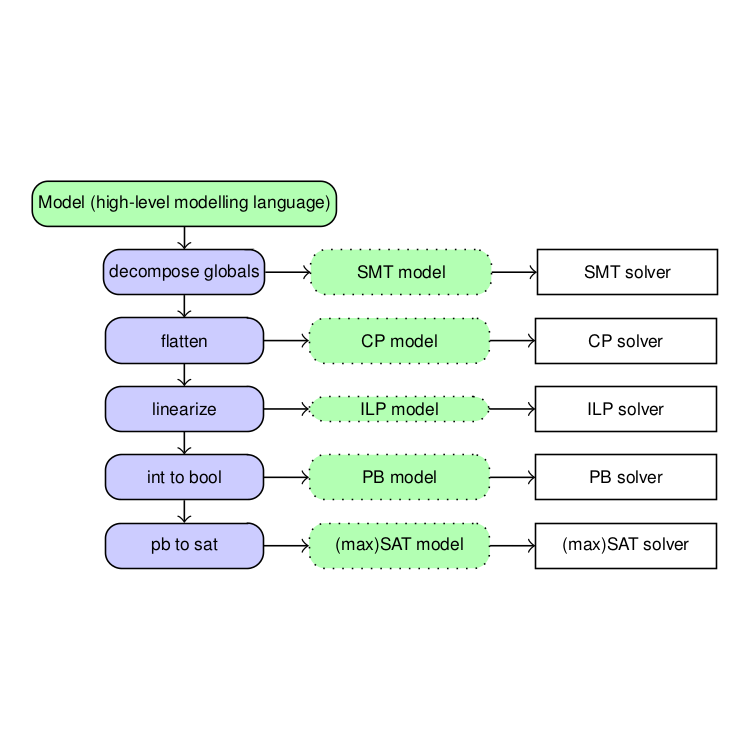
\includegraphics[height=35mm, trim=30px 30px 30px 30px, clip]{images/ch6-logo.png}
  \end{center}
  \vfill

  Better understand what a solver CAN do, and what it is GOOD at (or bad).
  \begin{itemize}
    \item CP: recommended if you have many global constraints
    \item ILP: recommended if many linear constraints and optimizing the 'continuous relaxation' is meaningful
    \item SMT: recommended if many disjunctive constraints (SAT reasoning + LIA reasoning)
  \end{itemize}
  

  (but there is no rulebook, recommended to try multiple solvers)
\end{frame}

\subsection*{Pseudo-Boolean (PB) Optimization}
% OVERVIEW: PB solver highlight
\begin{frame}{Overview}
\begin{tikzpicture}[scale=0.7, every node/.style={transform shape}, node distance=0.5cm]

% Model (green box)
\node[draw, fill=green!30, rounded corners, minimum width=2cm, minimum height=1cm] (model) {Model  (high-level modelling language)};

% Decompose-globals (blue box)
\node[draw, fill=blue!20, below=of model, rounded corners, minimum width=3.5cm, minimum height=1cm] (decompose) {decompose globals};
% Flatten (orange box)
\node[draw, fill=blue!20, below=of decompose, rounded corners, minimum width=3.5cm, minimum height=1cm] (flatten) {flatten};
% Linearize (purple box)
\node[draw, fill=blue!20, below=of flatten, rounded corners, minimum width=3.5cm, minimum height=1cm] (linearize) {linearize};
% int2bool (cyan box)
\node[draw, fill=blue!20, below=of linearize, rounded corners, minimum width=3.5cm, minimum height=1cm] (int2bool) {int to bool};
% pb2sat (pink box)
\node[draw, fill=blue!20, below=of int2bool, rounded corners, minimum width=3.5cm, minimum height=1cm] (pb2sat) {pb to sat};

% Low-level mdoels (no fill)
\node[draw, fill=green!30, rounded corners, dotted, minimum height=1cm, minimum width=4cm, right=1cm of decompose, align=left] (smt) {SMT model};
\node[draw, fill=green!30, rounded corners, dotted, minimum height=1cm, minimum width=4cm, right=1cm of flatten, align=left] (cp) {CP model};
\node[draw, fill=green!30, rounded corners, dotted, minimum width=4cm, right=1cm of linearize, fill=green!30, rounded corners, align=left] (ilp) {ILP model};
\node[draw, fill=green!30, rounded corners, dotted, minimum height=1cm, minimum width=4cm, right=1cm of int2bool, align=left] (pb) {PB model};
\node[draw, fill=green!30, rounded corners, dotted, minimum height=1cm, minimum width=4cm, right=1cm of pb2sat, align=left] (sat) {(max)SAT model};

% Solvers (no fill)
\node[draw, minimum height=1cm, minimum width=4cm, right=1cm of smt, align=left] (smt2) {SMT solver};
\node[draw, minimum height=1cm, minimum width=4cm, right=1cm of cp, align=left] (cp2) {CP solver};
\node[draw, minimum height=1cm, minimum width=4cm, right=1cm of ilp, align=left] (ilp2) {ILP solver};
\node[draw, fill=red!30, minimum height=1cm, minimum width=4cm, right=1cm of pb, align=left] (pb2) {PB solver};
\node[draw, minimum height=1cm, minimum width=4cm, right=1cm of sat, align=left] (sat2) {(max)SAT solver};

% Arrows
\draw[->] (model) -- (decompose); 
\draw[->] (decompose) -- (flatten);
\draw[->] (flatten) -- (linearize);
\draw[->] (linearize) -- (int2bool);
\draw[->] (int2bool) -- (pb2sat);

% Connections to low-level
\draw[->] (decompose.east) -- ++(0.5,0) |- (smt.west);
\draw[->] (flatten.east) -- ++(0.5,0) |- (cp.west);
\draw[->] (linearize.east) -- ++(0.5,0) |- (ilp.west);
\draw[->] (int2bool.east) -- ++(0.5,0) |- (pb.west);
\draw[->] (pb2sat.east) -- ++(0.5,0) |- (sat.west);

% Connections to solvers
\draw[->] (smt.east) -- ++(0.5,0) |- (smt2.west);
\draw[->] (cp.east) -- ++(0.5,0) |- (cp2.west);
\draw[->] (ilp.east) -- ++(0.5,0) |- (ilp2.west);
\draw[->] (pb.east) -- ++(0.5,0) |- (pb2.west);
\draw[->] (sat.east) -- ++(0.5,0) |- (sat2.west);

\end{tikzpicture}
\end{frame}


\begin{frame}{Pseudo-Boolean (PB) Optimization}
  \begin{itemize}
    \item \textbf{Pseudo-Boolean Constraints}: $\sum_{i=1}^n a_i x_i \leq b$, where $a_i, b$ are integers and $x_i$ are Boolean variables.
    \item Solves combinatorial optimization problems where the objective function and constraints are \textbf{linear} and only involve \textbf{Boolean variables} (0-1 variables)
    \item Extends SAT by allowing linear inequalities over Boolean variables
    %\item Can handle both \textit{satisfaction} and \textit{optimization} problems
  \end{itemize}
  \vfill

  \textbf{How it Works (High-Level Overview)} $ $\\
  \begin{enumerate}
    \item Either encode into SAT (see next part);
    \item Or use native pseudo-boolean cutting plane solving (not covered in lecture)
  \end{enumerate}
  \vspace{0.4cm}

  \textbf{Typical Applications}
  \begin{itemize}
    \item Hardware/software verification, Circuit design
    \item Resource allocation, Packing problems
    \item Scheduling, Timetabling, Logistics
  \end{itemize}
\end{frame}


\subsection*{Transformation: int to bool}
\begin{frame}{Overview}
\begin{tikzpicture}[scale=0.7, every node/.style={transform shape}, node distance=0.5cm]

% Model (green box)
\node[draw, fill=green!30, rounded corners, minimum width=2cm, minimum height=1cm] (model) {Model  (high-level modelling language)};

% Decompose-globals (blue box)
\node[draw, fill=blue!20, below=of model, rounded corners, minimum width=3.5cm, minimum height=1cm] (decompose) {decompose globals};
% Flatten (orange box)
\node[draw, fill=blue!20, below=of decompose, rounded corners, minimum width=3.5cm, minimum height=1cm] (flatten) {flatten};
% Linearize (purple box)
\node[draw, fill=blue!20, below=of flatten, rounded corners, minimum width=3.5cm, minimum height=1cm] (linearize) {linearize};
% int2bool (cyan box)
\node[draw, fill=red!30, below=of linearize, rounded corners, minimum width=3.5cm, minimum height=1cm] (int2bool) {int to bool};
% pb2sat (pink box)
\node[draw, fill=blue!20, below=of int2bool, rounded corners, minimum width=3.5cm, minimum height=1cm] (pb2sat) {pb to sat};

% Low-level mdoels (no fill)
\node[draw, fill=green!30, rounded corners, dotted, minimum height=1cm, minimum width=4cm, right=1cm of decompose, align=left] (smt) {SMT model};
\node[draw, fill=green!30, rounded corners, dotted, minimum height=1cm, minimum width=4cm, right=1cm of flatten, align=left] (cp) {CP model};
\node[draw, fill=green!30, rounded corners, dotted, minimum width=4cm, right=1cm of linearize, fill=green!30, rounded corners, align=left] (ilp) {ILP model};
\node[draw, fill=green!30, rounded corners, dotted, minimum height=1cm, minimum width=4cm, right=1cm of int2bool, align=left] (pb) {PB model};
\node[draw, fill=green!30, rounded corners, dotted, minimum height=1cm, minimum width=4cm, right=1cm of pb2sat, align=left] (sat) {(max)SAT model};

% Solvers (no fill)
\node[draw, minimum height=1cm, minimum width=4cm, right=1cm of smt, align=left] (smt2) {SMT solver};
\node[draw, minimum height=1cm, minimum width=4cm, right=1cm of cp, align=left] (cp2) {CP solver};
\node[draw, minimum height=1cm, minimum width=4cm, right=1cm of ilp, align=left] (ilp2) {ILP solver};
\node[draw, minimum height=1cm, minimum width=4cm, right=1cm of pb, align=left] (pb2) {PB solver};
\node[draw, minimum height=1cm, minimum width=4cm, right=1cm of sat, align=left] (sat2) {(max)SAT solver};

% Arrows
\draw[->] (model) -- (decompose); 
\draw[->] (decompose) -- (flatten);
\draw[->] (flatten) -- (linearize);
\draw[->] (linearize) -- (int2bool);
\draw[->] (int2bool) -- (pb2sat);

% Connections to low-level
\draw[->] (decompose.east) -- ++(0.5,0) |- (smt.west);
\draw[->] (flatten.east) -- ++(0.5,0) |- (cp.west);
\draw[->] (linearize.east) -- ++(0.5,0) |- (ilp.west);
\draw[->] (int2bool.east) -- ++(0.5,0) |- (pb.west);
\draw[->] (pb2sat.east) -- ++(0.5,0) |- (sat.west);

% Connections to solvers
\draw[->] (smt.east) -- ++(0.5,0) |- (smt2.west);
\draw[->] (cp.east) -- ++(0.5,0) |- (cp2.west);
\draw[->] (ilp.east) -- ++(0.5,0) |- (ilp2.west);
\draw[->] (pb.east) -- ++(0.5,0) |- (pb2.west);
\draw[->] (sat.east) -- ++(0.5,0) |- (sat2.west);

\end{tikzpicture}
\end{frame}


\begin{frame}{Encoding into (pseudo)Boolean constraints}
  \structured{Challenges:}
  \begin{itemize}
    \item How to encode an integer variable into a collection of Boolean
      variables?
    \item How to encode a constraint on integer variables into (a
      collection of) constraints on Boolean variables?
  \end{itemize}
  \vfill

  \structured{Considerations:}
  \begin{itemize}
    \item We want few variables.
    \item We want few constraints, or short constraints.
  \end{itemize}
  \vfill%

  As usual, there are many possibilities and it is not always clear
  what the best choice is.
\end{frame}

\begin{frame}{Encoding an Integer Variable}
  Well-known encodings, described on the next slides: \vfill
  \begin{itemize}
    \item \defined{Direct (or sparse or one-hot) encoding}: \\
      a Boolean 'equality' variable for each value in the domain. \vfill
    \item \defined{Order encoding}: \\
      a Boolean 'inequality' variable for each value in the domain. \vfill
    \item \defined{Bit (or binary or log) encoding}: \\
      a Boolean variable for each bit in the base-2 representation of
      the largest domain value.
  \end{itemize}
\end{frame}

\begin{frame}{\defined{Direct} Encoding of an Integer Variable}
  Consider an integer variable $x$ with domain $1..n$: \vfill
  \begin{itemize}
    \item Create a Boolean variable $b_{[x=k]}$ for all $k \in \{1..n\}$
      \vfill
    \item The variable $b_{[x=k]}$ is \textbf{true} if and only if
      $x = k$ holds \vfill
    \item Consistency constraint: \vfill
      \begin{itemize}
          \item Variable $x$ has exactly one value from domain: $\sum_{k \in \{1..n\}} (b_{[x=k]}) = 1$\vfill
      \end{itemize} \vfill
    \item Example encodings of simple constraints:
      \begin{itemize}
        \item The constraint $x \neq k$ is encoded as $\lnot b_{[x=k]}$.
          \vfill
        \item The constraint $x < k$ is encoded as
          $\displaystyle\bigwedge_{j \in k..n} \lnot b_{[x=j]}$.
        \item In any constraint, can replace $x$ by $\sum_k k*b_{[x=k]}$
      \end{itemize}
  \end{itemize}
\end{frame}

\begin{frame}{\defined{Order} Encoding of an Integer Variable}
  Consider an integer variable $x$ with domain $1..n$: \vfill
  \begin{itemize}
    \item Create a Boolean variable $b_{[x \geq k]}$ for all $k$ in
      $1..(n+1)$. \vfill
    \item The variable $b_{[x \geq k]}$ is \textbf{true} if and only if
      $x \geq k$ holds. \vfill
    \item Consistency constraints: \vfill
      \begin{itemize}
        \item Order:
          $\displaystyle\bigwedge_{k \in 1..n} \left(b_{[x \geq k+1]} \rightarrow b_{[x \geq k]} \right)$ \vfill
        \item Bounds of domain: $b_{[x \geq 1]} \land \lnot b_{[x \geq n+1]}$
      \end{itemize} \vfill
    \item Example encodings of simple constraints:
      \begin{itemize}
        \item The constraint $x = k$ is encoded as
          $b_{[x \geq k]} \land \lnot b_{[x \geq k+1]}$. \vfill
        \item The constraint $x \neq k$ is encoded as
          $\lnot b_{[x \geq k]} \lor b_{[x \geq k+1]}$. \vfill
        %\item The constraint $x < k$ is encoded as $\lnot b_{[x \geq k]}$.
        \item In any constraint, can replace $x$ by $\sum_k b_{[x \geq k]}$.
      \end{itemize}
  \end{itemize}
\end{frame}

\begin{frame}{\defined{Log} Encoding of an Integer Variable}
  Consider an integer variable $x$ with domain $1..n$: \vfill
  \begin{itemize}
    \item Encode the value of $x$ in binary, using just $\lceil \log_2(n) \rceil$ Boolean variables. \vfill
    \item Let $b_i$ be a Boolean variable representing the $i$-th bit in the binary encoding of $x$. \vfill
    \item In any constraint, can replace $x$ by (note that the lowest value for x is 1):
      \[
      x = 1 + \sum_{i=0}^{\lceil \log_2(n) \rceil - 1} b_i \cdot 2^i
      \]
      where $b_i \in \{0, 1\}$. \vfill
    \item Consistency constraint: 
      \begin{itemize}
        \item Upper bound of domain:  $1 + \sum_{i=0}^{\lceil \log_2(n) \rceil - 1} b_i \cdot 2^i \leq n$ (in case $n$ is not a power of 2)
      \end{itemize}
      %
    %\item This encoding requires $\lceil \log_2(n) \rceil$ Boolean variables and a few additional constraints if $n$ is not a power of 2. \vfill
    %\item The constraint $x = k$ is encoded by setting the binary variables to match the binary representation of $k$. \vfill
    %\item The constraint $x \neq k$ is encoded by ensuring at least one bit in the binary representation of $x$ differs from that of $k$. \vfill
    %\item Constraints for inequalities like $x < k$ or $x > k$ can also be derived by comparing binary representations.
  \end{itemize}
\end{frame}

\begin{frame}{Encodings: example with overview}
  \centering
  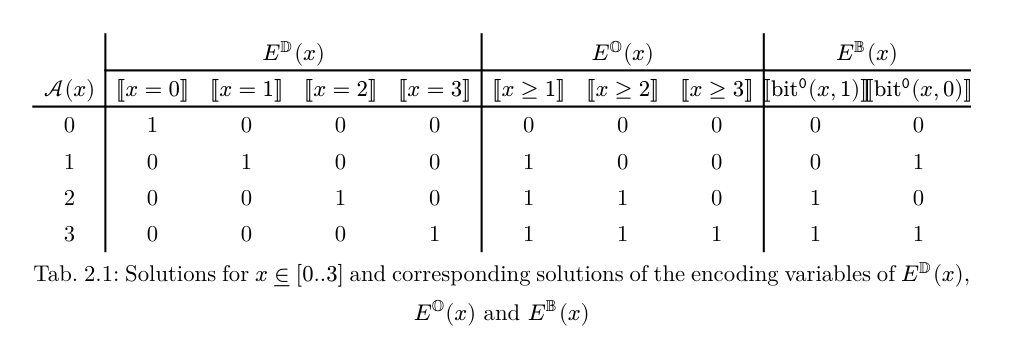
\includegraphics[width=\columnwidth]{images/encodings}
\end{frame}

\subsection*{Boolean Satisfiability (SAT/MaxSAT)}
% OVERVIEW: SAT solver highlight
\begin{frame}{Overview}
\begin{tikzpicture}[scale=0.7, every node/.style={transform shape}, node distance=0.5cm]

% Model (green box)
\node[draw, fill=green!30, rounded corners, minimum width=2cm, minimum height=1cm] (model) {Model  (high-level modelling language)};

% Decompose-globals (blue box)
\node[draw, fill=blue!20, below=of model, rounded corners, minimum width=3.5cm, minimum height=1cm] (decompose) {decompose globals};
% Flatten (orange box)
\node[draw, fill=blue!20, below=of decompose, rounded corners, minimum width=3.5cm, minimum height=1cm] (flatten) {flatten};
% Linearize (purple box)
\node[draw, fill=blue!20, below=of flatten, rounded corners, minimum width=3.5cm, minimum height=1cm] (linearize) {linearize};
% int2bool (cyan box)
\node[draw, fill=blue!20, below=of linearize, rounded corners, minimum width=3.5cm, minimum height=1cm] (int2bool) {int to bool};
% pb2sat (pink box)
\node[draw, fill=blue!20, below=of int2bool, rounded corners, minimum width=3.5cm, minimum height=1cm] (pb2sat) {pb to sat};

% Low-level mdoels (no fill)
\node[draw, fill=green!30, rounded corners, dotted, minimum height=1cm, minimum width=4cm, right=1cm of decompose, align=left] (smt) {SMT model};
\node[draw, fill=green!30, rounded corners, dotted, minimum height=1cm, minimum width=4cm, right=1cm of flatten, align=left] (cp) {CP model};
\node[draw, fill=green!30, rounded corners, dotted, minimum width=4cm, right=1cm of linearize, fill=green!30, rounded corners, align=left] (ilp) {ILP model};
\node[draw, fill=green!30, rounded corners, dotted, minimum height=1cm, minimum width=4cm, right=1cm of int2bool, align=left] (pb) {PB model};
\node[draw, fill=green!30, rounded corners, dotted, minimum height=1cm, minimum width=4cm, right=1cm of pb2sat, align=left] (sat) {(max)SAT model};

% Solvers (no fill)
\node[draw, minimum height=1cm, minimum width=4cm, right=1cm of smt, align=left] (smt2) {SMT solver};
\node[draw, minimum height=1cm, minimum width=4cm, right=1cm of cp, align=left] (cp2) {CP solver};
\node[draw, minimum height=1cm, minimum width=4cm, right=1cm of ilp, align=left] (ilp2) {ILP solver};
\node[draw, minimum height=1cm, minimum width=4cm, right=1cm of pb, align=left] (pb2) {PB solver};
\node[draw, fill=red!30, minimum height=1cm, minimum width=4cm, right=1cm of sat, align=left] (sat2) {(max)SAT solver};

% Arrows
\draw[->] (model) -- (decompose); 
\draw[->] (decompose) -- (flatten);
\draw[->] (flatten) -- (linearize);
\draw[->] (linearize) -- (int2bool);
\draw[->] (int2bool) -- (pb2sat);

% Connections to low-level
\draw[->] (decompose.east) -- ++(0.5,0) |- (smt.west);
\draw[->] (flatten.east) -- ++(0.5,0) |- (cp.west);
\draw[->] (linearize.east) -- ++(0.5,0) |- (ilp.west);
\draw[->] (int2bool.east) -- ++(0.5,0) |- (pb.west);
\draw[->] (pb2sat.east) -- ++(0.5,0) |- (sat.west);

% Connections to solvers
\draw[->] (smt.east) -- ++(0.5,0) |- (smt2.west);
\draw[->] (cp.east) -- ++(0.5,0) |- (cp2.west);
\draw[->] (ilp.east) -- ++(0.5,0) |- (ilp2.west);
\draw[->] (pb.east) -- ++(0.5,0) |- (pb2.west);
\draw[->] (sat.east) -- ++(0.5,0) |- (sat2.west);

\end{tikzpicture}
\end{frame}


\begin{frame}{Boolean Satisfiability (SAT) / Max-SAT}
  \begin{itemize}
    \item Determines the satisfiability of a propositional logic formula over Boolean variables, typically expressed in conjunctive normal form (CNF)
    \item A solution is a complete assignment that satisfies the formula
    \item Max-SAT extends SAT by maximizing the number of satisfied clauses in cases where not all clauses can be satisfied
  \end{itemize}
  \vfill

  \textbf{How it Works (High-Level Overview)} $ $\\
  %Utilizes search algorithms and learning techniques.
  \begin{itemize}
    \item \textbf{DPLL Algorithm} systematically explores variable assignments and backtracks upon conflicts
    \item \textbf{Conflict-Driven Clause Learning (CDCL)} captures conflicts to avoid repeating mistakes in future search
  \end{itemize}
  \vfill

  \textbf{Typical Applications}
  \begin{itemize}
    \item Hardware/software verification, Model checking
    \item Planning and Resource allocation
  \end{itemize}
\end{frame}


\begin{frame}[fragile]{Boolean Satisfiability Solving (SAT)}
  \structured{Modelling Language:}
  \begin{itemize}
    \item Only Boolean decision variables.
    \item CNF is a conjunction ($\land$) of clauses.
      A \defined{clause} is a disjunction ($\lor)$ of literals.
      A~\defined{literal} is a Boolean decision variable ($x$) or its negation
      ($\neg x$).
    \item Only for satisfaction problems; else: MaxSAT.
  \end{itemize}
  \vfill

  \begin{example}
    \begin{itemize}
      \item Boolean decision variables: w, x, y, z
      \item Clauses:
      \begin{align*}
        (\neg w \lor \neg y) \land (\neg x \lor y) \land
        (\neg w \lor x \lor \neg z) \\ \land (x \lor y \lor z) \land
        (w \lor \neg z)
      \end{align*}
      \item A solution: $w=$ False,
        $x=$ True, $y=$ True, $z=$ False
    \end{itemize}
  \end{example}
\end{frame}

\begin{flashcardcpmpy}
\begin{frame}[fragile]{Boolean Satisfiability Solving (SAT) -- CPMpy}
  \structured{Modelling Language:}
  \begin{itemize}
    \item Only Boolean decision variables.
    \item CNF is a conjunction ($\land$) of clauses.
      A \defined{clause} is a disjunction ($\lor)$ of literals.
      A~\defined{literal} is a Boolean decision variable ($x$) or its negation
      ($\neg x$).
    \item Only for satisfaction problems; else: MaxSAT.
  \end{itemize}
  \vfill

  \begin{example}[in CPMpy]
    \begin{itemize}
      \item Decision variables: \cpminline{ w, x, y, z = cp.boolvar(shape=4)}
      \item Clauses:
        \begin{cpmno}
  model += (~w | ~y) & (~x | y) & (~w | x | ~z) \
          & (x | y | z) & (w | ~z)
        \end{cpmno}
      \item A solution: \cpminline{w=False},
        \cpminline{x=True}, \cpminline{y=True}, \cpminline{z=False}
    \end{itemize}
  \end{example}
\end{frame}
\end{flashcardcpmpy}

\begin{frame}{The SAT Problem}
  Given a clause set, find an \defined{assignment}, that is, Boolean
  values for all the decision variables, so that all the clauses are
  satisfied. \vfill
  \begin{itemize}
    \item The decision version of this problem is NP-complete. \vfill
    \item \alert{Any combinatorial problem can be encoded into SAT.} \\
      Careful: ``encoded into'' is not ``reduced from'', but ``reduced
      to''. \\
      It might require an exponential number of constraints...
      \vfill
    \item There has been intensive research on SAT solving since the 1960s, and still very active with yearly competitions. \vfill
    \item Most modern SMT/CP/PB solvers are built on/include a SAT solver.\vfill
  \end{itemize}
\end{frame}

\begin{frame}{DPLL [Davis-Putnam-Logemann-Loveland, 1962]}
  \inference{Inference:}
  \begin{itemize}
    \item \defined{Unit propagation}: If all the literals in a clause
      evaluate to \mzninline{false}, \\ except one whose decision
      variable has no value yet, then that literal is made to evaluate
      to \mzninline{true} so that the clause becomes satisfied.\\
      Example: $x \lor \neg y \lor \neg z$ with $x=F$ and $y=T$ propagates $z=...$
  \end{itemize}
  
  \search{Tree Search}: (start with empty valuation)
  \begin{enumerate}
    \item Perform \inference{inference}, e.g. unit propagation
    \item If some clause is unsatisfied, then backtrack.
    \item If all decision variables have a value, then we have a
      solution.
    \item Select an unvalued decision variable $b$ and make two branches: \\
      one with $b = \mzninline{true}$, and the other one with
      $b = \mzninline{false}$.
    \item Recursively explore each of the two branches.
  \end{enumerate}\vfill%
\end{frame}

\begin{frame}{Strategies and Improvements over DPLL}\label{sat}
  \search{Search Strategies:}
  \begin{itemize}
    \item On which decision variable to branch next?
    \item Which branch to explore next?
    \item Which search (depth-first, breadth-first, \dots) to use?
  \end{itemize}\vfill%
  \structured{Improvements:}
  \begin{itemize}
    \item \inference{Clause learning}: on failure, analyse the conflict and learn a new clause from it
    \item \search{Backjumping}: backtrack multiple levels at once (based on learned clause)
    \item \search{Restarts}: backjump to root node (valid due to learned clauses)
    \item A lot of implementation details, e.g. data structures
    \item \dots
  \end{itemize}
\end{frame}

\begin{frame}{SAT Solving}
  \begin{itemize}
    \item Guarantee: exact, given enough time. \vfill
    \item Mainly black-box: there are limited ways to guide the solving.
      \vfill
    \item It can scale to millions of decision variables and clauses.
      \vfill
    \item Encoding a problem can yield a huge SAT model. \vfill
    \item For debugging and explanation purposes, solvers can extract an
      \defined{unsatisfiable core}, that is a subset of the clauses that
      make the model unsatisfiable. \vfill
    \item It is mainly applied in hardware verification and software
      verification.
  \end{itemize}
\end{frame}


\subsection*{Transformation: pb to sat}
\begin{frame}{Overview}
\begin{tikzpicture}[scale=0.7, every node/.style={transform shape}, node distance=0.5cm]

% Model (green box)
\node[draw, fill=green!30, rounded corners, minimum width=2cm, minimum height=1cm] (model) {Model  (high-level modelling language)};

% Decompose-globals (blue box)
\node[draw, fill=blue!20, below=of model, rounded corners, minimum width=3.5cm, minimum height=1cm] (decompose) {decompose globals};
% Flatten (orange box)
\node[draw, fill=blue!20, below=of decompose, rounded corners, minimum width=3.5cm, minimum height=1cm] (flatten) {flatten};
% Linearize (purple box)
\node[draw, fill=blue!20, below=of flatten, rounded corners, minimum width=3.5cm, minimum height=1cm] (linearize) {linearize};
% int2bool (cyan box)
\node[draw, fill=blue!20, below=of linearize, rounded corners, minimum width=3.5cm, minimum height=1cm] (int2bool) {int to bool};
% pb2sat (pink box)
\node[draw, fill=red!30, below=of int2bool, rounded corners, minimum width=3.5cm, minimum height=1cm] (pb2sat) {pb to sat};

% Low-level mdoels (no fill)
\node[draw, fill=green!30, rounded corners, dotted, minimum height=1cm, minimum width=4cm, right=1cm of decompose, align=left] (smt) {SMT model};
\node[draw, fill=green!30, rounded corners, dotted, minimum height=1cm, minimum width=4cm, right=1cm of flatten, align=left] (cp) {CP model};
\node[draw, fill=green!30, rounded corners, dotted, minimum width=4cm, right=1cm of linearize, fill=green!30, rounded corners, align=left] (ilp) {ILP model};
\node[draw, fill=green!30, rounded corners, dotted, minimum height=1cm, minimum width=4cm, right=1cm of int2bool, align=left] (pb) {PB model};
\node[draw, fill=green!30, rounded corners, dotted, minimum height=1cm, minimum width=4cm, right=1cm of pb2sat, align=left] (sat) {(max)SAT model};

% Solvers (no fill)
\node[draw, minimum height=1cm, minimum width=4cm, right=1cm of smt, align=left] (smt2) {SMT solver};
\node[draw, minimum height=1cm, minimum width=4cm, right=1cm of cp, align=left] (cp2) {CP solver};
\node[draw, minimum height=1cm, minimum width=4cm, right=1cm of ilp, align=left] (ilp2) {ILP solver};
\node[draw, minimum height=1cm, minimum width=4cm, right=1cm of pb, align=left] (pb2) {PB solver};
\node[draw, minimum height=1cm, minimum width=4cm, right=1cm of sat, align=left] (sat2) {(max)SAT solver};

% Arrows
\draw[->] (model) -- (decompose); 
\draw[->] (decompose) -- (flatten);
\draw[->] (flatten) -- (linearize);
\draw[->] (linearize) -- (int2bool);
\draw[->] (int2bool) -- (pb2sat);

% Connections to low-level
\draw[->] (decompose.east) -- ++(0.5,0) |- (smt.west);
\draw[->] (flatten.east) -- ++(0.5,0) |- (cp.west);
\draw[->] (linearize.east) -- ++(0.5,0) |- (ilp.west);
\draw[->] (int2bool.east) -- ++(0.5,0) |- (pb.west);
\draw[->] (pb2sat.east) -- ++(0.5,0) |- (sat.west);

% Connections to solvers
\draw[->] (smt.east) -- ++(0.5,0) |- (smt2.west);
\draw[->] (cp.east) -- ++(0.5,0) |- (cp2.west);
\draw[->] (ilp.east) -- ++(0.5,0) |- (ilp2.west);
\draw[->] (pb.east) -- ++(0.5,0) |- (pb2.west);
\draw[->] (sat.east) -- ++(0.5,0) |- (sat2.west);

\end{tikzpicture}
\end{frame}


\begin{frame}{Encoding PB to SAT}
  Example: $\sum_{k \in \{1..n\}} b_{k} = 1$ (as used e.g. in the direct encoding of integers)

  \begin{align}
    \sum_{k \in \{1..n\}} b_{k} = 1 &\Leftrightarrow
        \sum_{k \in \{1..n\}} b_{k} \geq 1 ~\wedge~
        \sum_{k \in \{1..n\}} b_{k} \leq 1 \\
    \sum_{k \in \{1..n\}} b_{k} \geq 1 &\Leftrightarrow
          \bigvee_{k \in 1..n} b_k \\
    \sum_{k \in \{1..n\}} b_{k} \leq 1 
      & \Leftrightarrow \bigwedge_{i,j \in 1..n,~ i < j} \left(b_i + b_j \leq 1\right) \\
      & \Leftrightarrow \bigwedge_{i,j \in 1..n,~ i < j} \left(\neg b_i \lor \neg b_j\right)
  \end{align}

  From 1 PB constraint over $m$ variables, \\
  to 1 clause over $m$ variables + $m*(m-1)/2$ binary clauses.
\end{frame}

\begin{frame}{Encoding any PB Constraint to SAT}
  \small
  \textbf{Pseudo-Boolean Constraints}: $\sum_{i=1}^n a_i x_i \leq b$, with $a_i, b$ integers, $x_i$ Boolean variables.
  \vfill

  Many encoding techniques exist, e.g.: (details beyond the scope of this course)
  \begin{itemize}
    \item \textbf{Adder Networks:}
      \begin{itemize}
        \item Use a network of binary adder circuits (like in hardware) to encode the sum.
        \item Network is polynomial in size, but has weaker propagation (not \textit{arc consistent}).
      \end{itemize}
        
    \item \textbf{Sorting Networks:}
      \begin{itemize}
        \item Use a network of comparators to sort inputs, enforcing PB constraints on sums.
        \item Strong propagation \& works well for small/medium $n$, but often exponential size.
      \end{itemize}

    \item \textbf{Totalizer Encoding:}
      \begin{itemize}
        \item Introduces auxiliary variables for cumulative sums.
        \item Useful for incremental solving; strong propagation but at worst exponential size.
      \end{itemize}
        
    \item \textbf{Binary Decision Diagrams (BDD):}
      \begin{itemize}
        \item Use a BDD over the $x_i$s to compactly represent the allowed values.
        \item Strong propagation, but building BDDs can be computationally expensive \& worst-case exponential size.
      \end{itemize}\vfill
  \end{itemize}
\end{frame}


\section*{Choosing a Technology and Backend}

\begin{frame}{Choosing a Solver Technology}
  \begin{itemize}
    \item Do you need guarantees that a found solution is optimal, \\
      that all solutions are found, and that unsatisfiability is
      provable? \vfill
    \item What types of decision variables are in your model? \vfill
    \item What constraint predicates are in your model? \vfill
    \item Does your problem look like a well-known problem? \vfill
    \item How do backends perform on easy problem instances? \vfill
    \item What is your favourite technology or backend?
  \end{itemize}
\end{frame}

\begin{frame}{Some Caveats}
  \begin{itemize}
    \item Each problem can be modelled in many different ways.
    \item Different models of the same problem are better suited for different
      backends.
    \item Performance on small instances does not always scale to larger
      instances.
    \item Sometimes, a good \search{search strategy} is more important
      than a good model (see next lecture).
    \item Not all backends of the same technology have comparable
      performance.
    \item Some pure problems can be solved by specialist solvers, \\
      such as
      \href{https://www.math.uwaterloo.ca/tsp/concorde}{Concorde} for
      the travelling salesperson problem, \\ but real-life side
      constraints often make them inapplicable.
    \item Some problems are maybe even solvable in polynomial time and
      space.
  \end{itemize}
\end{frame}

\begin{frame}
  \structured{Take-Home Message:}
  \begin{itemize}
    \item There are many solving technologies and backends.
    \item It is useful to highlight the commonalities and differences.
    \item No solving technology or backend can be universally better
      than all the others, unless $\textnormal{P} = \textnormal{NP}$.
  \end{itemize}
  \begin{center}
    \handpoint\ With solver-independent frameworks: can try multiple ones!
  \end{center}

  \structured{To go further:} \\
  \begin{thebibliography}{99}
    \beamertemplatebookbibitems
  \bibitem{hooker} John N. Hooker. \\
    \href{https://link.springer.com/book/10.1007\%2F978-1-4614-1900-6}{Integrated Methods for Optimization}. \\
    2nd edition, Springer, 2012.
  \end{thebibliography}
\end{frame}

\end{document}
